\documentclass[tikz,border=5mm]{standalone}
\usetikzlibrary{matrix,positioning,arrows.meta,fit}

\begin{document}
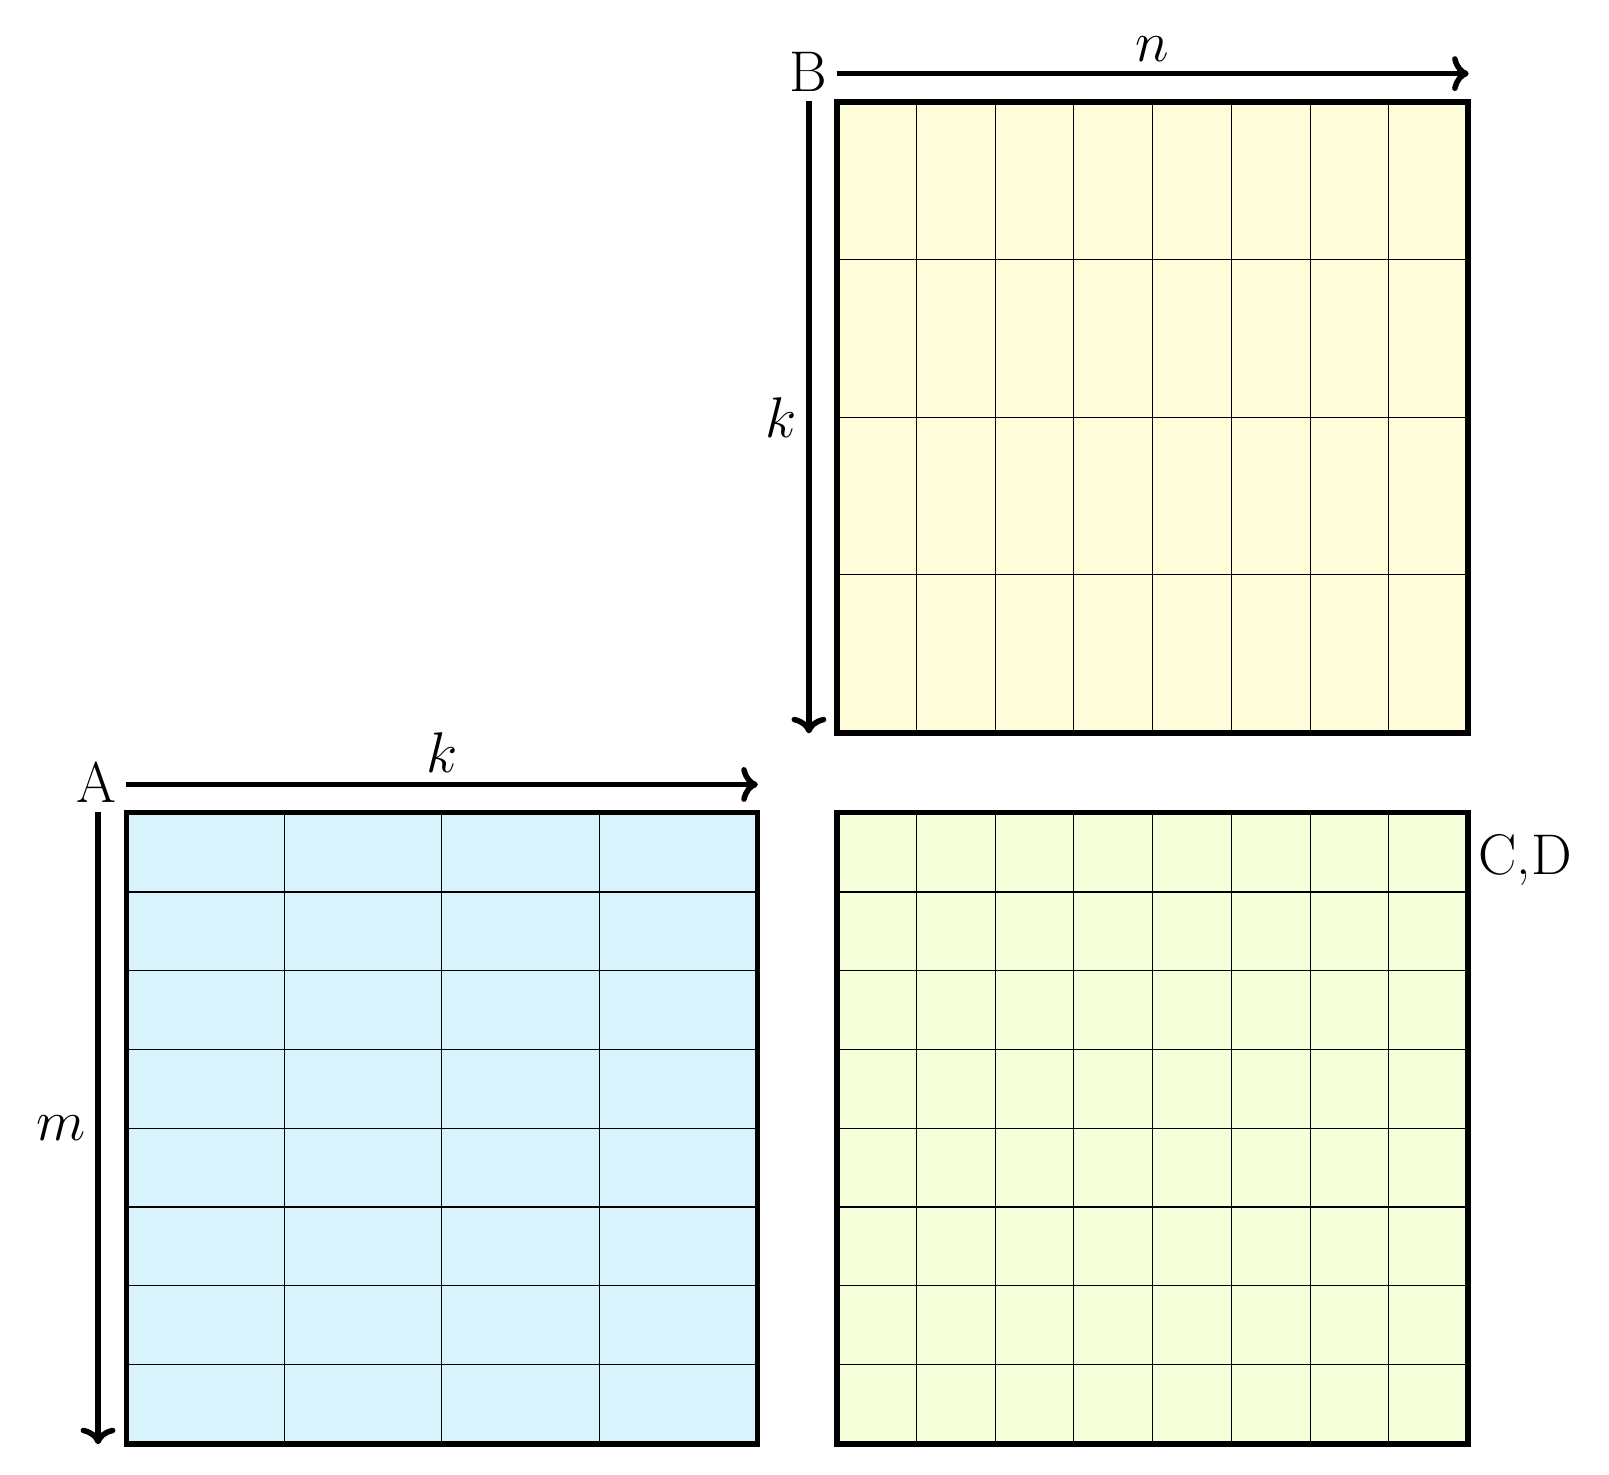
\begin{tikzpicture}[
    amatrix/.style={
        matrix of nodes,
        nodes={
            draw,
            minimum height=1cm,
            minimum width=2cm,
            anchor=center
            },
        column sep=-\pgflinewidth,
        row sep=-\pgflinewidth,
        inner sep=0pt
    },
    bmatrix/.style={
        matrix of nodes,
        nodes={
            draw,
            minimum height=2cm,
            minimum width=1cm,
            anchor=center
            },
        column sep=-\pgflinewidth,
        row sep=-\pgflinewidth,
        inner sep=0pt
    },
    cmatrix/.style={
        matrix of nodes,
        nodes={
            draw,
            minimum height=1cm,
            minimum width=1cm,
            anchor=center
            },
        column sep=-\pgflinewidth,
        row sep=-\pgflinewidth,
        inner sep=0pt
    },
%    >=Stealth
]

% Matrix A (8x4 square)
\matrix[amatrix, fill=cyan!15, label={[name=A_label, font=\huge]above left:A}] (A) {
    |[fill=none]| & |[fill=none]| & |[fill=none]| & |[fill=none]| \\
    |[fill=none]| & |[fill=none]| & |[fill=none]| & |[fill=none]| \\
    |[fill=none]| & |[fill=none]| & |[fill=none]| & |[fill=none]| \\
    |[fill=none]| & |[fill=none]| & |[fill=none]| & |[fill=none]| \\
    |[fill=none]| & |[fill=none]| & |[fill=none]| & |[fill=none]| \\
    |[fill=none]| & |[fill=none]| & |[fill=none]| & |[fill=none]| \\
    |[fill=none]| & |[fill=none]| & |[fill=none]| & |[fill=none]| \\
    |[fill=none]| & |[fill=none]| & |[fill=none]| & |[fill=none]| \\
};

% Matrix C (8x8 square)
\matrix[cmatrix, fill=lime!15, right=of A.east, label={[name=C_label, font=\huge, yshift=-30pt]above right:C,D}] (C) {
    |[fill=none]| & |[fill=none]| & |[fill=none]| & |[fill=none]| & |[fill=none]| & |[fill=none]| & |[fill=none]| & |[fill=none]| \\
    |[fill=none]| & |[fill=none]| & |[fill=none]| & |[fill=none]| & |[fill=none]| & |[fill=none]| & |[fill=none]| & |[fill=none]| \\
    |[fill=none]| & |[fill=none]| & |[fill=none]| & |[fill=none]| & |[fill=none]| & |[fill=none]| & |[fill=none]| & |[fill=none]| \\
    |[fill=none]| & |[fill=none]| & |[fill=none]| & |[fill=none]| & |[fill=none]| & |[fill=none]| & |[fill=none]| & |[fill=none]| \\
    |[fill=none]| & |[fill=none]| & |[fill=none]| & |[fill=none]| & |[fill=none]| & |[fill=none]| & |[fill=none]| & |[fill=none]| \\
    |[fill=none]| & |[fill=none]| & |[fill=none]| & |[fill=none]| & |[fill=none]| & |[fill=none]| & |[fill=none]| & |[fill=none]| \\
    |[fill=none]| & |[fill=none]| & |[fill=none]| & |[fill=none]| & |[fill=none]| & |[fill=none]| & |[fill=none]| & |[fill=none]| \\
    |[fill=none]| & |[fill=none]| & |[fill=none]| & |[fill=none]| & |[fill=none]| & |[fill=none]| & |[fill=none]| & |[fill=none]| \\
};

% Matrix B (4x8 square)
\matrix[bmatrix, fill=yellow!15, above=of C.north, label={[name=B_label, font=\huge]above left:B}] (B) {
    |[fill=none]| & |[fill=none]| & |[fill=none]| & |[fill=none]| & |[fill=none]| & |[fill=none]| & |[fill=none]| & |[fill=none]| \\
    |[fill=none]| & |[fill=none]| & |[fill=none]| & |[fill=none]| & |[fill=none]| & |[fill=none]| & |[fill=none]| & |[fill=none]| \\
    |[fill=none]| & |[fill=none]| & |[fill=none]| & |[fill=none]| & |[fill=none]| & |[fill=none]| & |[fill=none]| & |[fill=none]| \\
    |[fill=none]| & |[fill=none]| & |[fill=none]| & |[fill=none]| & |[fill=none]| & |[fill=none]| & |[fill=none]| & |[fill=none]| \\
};

% draw outer boader
\node[draw,line width=2pt,inner sep=0pt,fit=(A-1-1)(A-8-4)] {};
\node[draw,line width=2pt,inner sep=0pt,fit=(B-1-1)(B-4-8)] {};
\node[draw,line width=2pt,inner sep=0pt,fit=(C-1-1)(C-8-8)] {};

% Arrows and labels
\draw[->, line width=2pt] ([xshift=-10pt]A.north west) -- ([xshift=-10pt]A.south west) node[midway, left, font=\huge] {$m$};
\draw[->, line width=2pt] ([yshift=10pt]A.north west) -- ([yshift=10pt]A.north east) node[midway, above, font=\huge] {$k$};
\draw[->, line width=2pt] ([xshift=-10pt]B.north west) -- ([xshift=-10pt]B.south west) node[midway, left, font=\huge] {$k$};
\draw[->, line width=2pt] ([yshift=10pt]B.north west) -- ([yshift=10pt]B.north east) node[midway, above, font=\huge] {$n$};

\end{tikzpicture}
\end{document}
